\documentclass[11pt]{article}

\usepackage{graphicx}
\newcommand{\head}[1]{\textnormal{\textbf{#1}}}
\begin{document}
    \begin{titlepage}
    \title {Design Document}
    \maketitle
        \begin{center}
		SE 2XA3\\
		\author{
		Hui Chen\hspace{128pt}chenh43	
		\\*Nareshkumar Maheshkumar\hspace{35pt}maheshn 
		\\*Sam Hamel\hspace{118pt}hamels2 \\
		}
		\end{center}
    \end{titlepage}
    
    \newpage
    
    \tableofcontents
    \listoffigures
    \listoftables
    
    \newpage
    \section{Revision History}
    \section{Module Guide For No Limit Texas HoldEm Program(NLTP)}
    \subsection{Introduction}
    \subsection{Anticipated and Unlikely Changes}
    \subsubsection{Anticipated Changes}
    \textbf{AC1}
     
    \subsubsection{Unlikely Changes}
    \textbf{UC1}
    
    \section{Module Hierarchy}
    \begin{table}[h]
    \caption{Module Hierarchy}
    \begin{tabular}{p{4cm}p{5cm}}
    \head{Level 1} & \head{Level 2} \\
    \hline
    Hardware Hiding & \\
    \hline
    Behaviour-Hiding  & TexasHoldEm Module \\
    Module & Pot Module\\
     & Game Module\\
    \hline
    Software Decision & Hand Module  \\
     & Deck Module\\
     & Player Module \\
     & AIOpponent Module\\
     & Card Module\\
    \hline
    \end{tabular}
    \end{table}
	
	\section{Connection Between Requirements and Design}
	\section{Module Decomposition}    
    \subsection{Hardware Hiding Module}
    \subsection{Behaviour-Hiding Module}
    \subsection{Software Decision Module}
    
    \section{MIS of TexasHoldEm Module}
    \subsection{Secret}
    \subsection{Service}
    \subsection{Exported Access Programs}
    \begin{table}[h]
    \caption{Exported Access Programs for TexasHoldEm Module}
    \begin{tabular}{p{4cm}p{2cm}p{2cm}p{4cm}}
    Name & In & Out & Exceptions\\
    \hline
	displayError() & int & - & Exception*\\
	\hline
    paint() & Graphic & - & -\\
    \hline
    save() & - & text file & FileNotFoundException\\
    \hline
    load() & text file & - & FileNotFoundException\\
    \hline
    actionPerformed() & ActionEvent &  - & - \\
    \hline
    \end{tabular}
    * all possible exceptions will be included, including but not limited to, FileNotFoundException and NullPointerException
    \end{table}
    
    \subsection{Interface Semantics}
    \subsubsection{State Variables}
    
    \subsubsection{Environment Variables}
	path:Location of the directory to be searched for when saving or loading the save file
	imagePath: Location of the directory to be searched for images of cards
    \subsubsection{Assumption}
    load() cannot be called without save() being called once before
    \subsubsection{Access Program Semantics}
    Main will populate the game window by instantiating the frame that is within TexasHoldEm module which will add all the components such as buttons, and uses paint() to populate the window with image of cards from environment variable imagePath and other simple graphics and colour for background. The save() will look for a save file in path. If it exists, it will overwrite it, if not, save() will create a new file. Load() will look for a save file in path and load all necessary data into the game and use Game module to modify the data for the affected modules. actionPerformed() will read the button input and call methods within Pot module based on its corresponding button. \\
    displayError():\\
    \textbf{Input} - Parameter of int type\\
    \textbf{transition} - Displays an error corresponding to the input  
    \newline
     \section{MIS of Pot Module}
     \subsection{Secret}
    \subsection{Service}
    \subsection{Exported Access Programs}
    \begin{table}[h]
    \caption{Exported Access Programs for Pot Module}
    \begin{tabular}{p{4cm}p{2cm}p{2cm}p{4cm}}
    Name & In & Out & Exceptions\\
    \hline
    anti() & - & - & -\\
    \hline
    call() & - & - & -\\
    \hline
    raise() & int & - & -\\
    \hline
    fold() & - & - & - \\
    \hline
    getBet() & - & int & NullPointerException\\
    \hline
    getPot() & - & int & -\\
    \hline
    roundEndEvaluate() & - & - & - \\
    \hline
    \end{tabular}
    \end{table}
    \subsection{Interface Semantics}
    \subsubsection{State Variables}
    pot:int\\
    bet:int\\
    player1:Player\\
    player2:Player
    \subsubsection{Environment Variables}
    \subsubsection{Assumption}
    \subsubsection{Access Program Semantics}
    anti uses the Player module to modify both players' chips and also modifies the state variable pot by the same amount taken from player's chips. Call() and raise() uses the Player module to modify corresponding player's chips by the amount read by TexasHoldEm module. Fold() uses the Game module to modify the corresponding playerFolded parameter and also uses Player module to modify the amount of chips lost or gained. roundEndEvaluate() uses Player module to modify the amount of chips and uses the Game module to initialize a new round. \\
    getPot():\\
    \textbf{Input} - No input required\\
    \textbf{Output} - Returns the value corresponding to the parameter pot\\
    getBet():\\
    \textbf{Input} - No input required\\
    \textbf{Output} - Returns the value corresponding to the parameter bet
    \newline
     \section{MIS of Game Module}
     \subsection{Secret}
    \subsection{Service}
    \subsection{Exported Access Programs}
    \begin{table}[h]
    \caption{Exported Access Programs for Game Module}
    \begin{tabular}{p{4cm}p{2cm}p{2cm}p{4cm}}
    Name & In & Out & Exceptions\\
    \hline
    playerSwitch() & - & - & -\\
    \hline
    deal() & - & - & -\\
    \hline
    nextCard() & - & - & -\\
    \hline
    isEndGame() & - & boolean & -\\
    \hline
    roundEnd() & - & - & - \\
    \hline
    player1Folded() & - & boolean & - \\
    \hline
    player2Folded() & - & boolean & - \\
    
    \end{tabular}
    \end{table}
    \subsection{Interface Semantics}
    \subsubsection{State Variables}
    currentPlayer:int\\
    Deck: list of Cards\\
    player1: Player\\
    player2: Player\\
    endGame: boolean\\
    player1Fold: boolean\\
    player2Fold: boolean
    \subsubsection{Environment Variables}
    \subsubsection{Assumption}
    \subsubsection{Access Program Semantics}
 	roundEnd() will call upon methods in Pot to evaluate, distribute the pot to the players and modify the parameters Deck, endGame, currentPlayer and each Player's hand by initializing the corresponding parameters as their default value or distribute new cards to the players.\\
 	playerSwitch():\\
 	\textbf{Input} - No input required\\
 	\textbf{transition} - modify currentPlayer between 2 values\\
 	deal():\\
 	\textbf{Input} - No input required\\
 	\textbf{Output} - Populates the Player hand variable\\
 	nextCard():\\
 	\textbf{Input} - No input required\\
 	\textbf{Output} - Modifies both players' hands by adding the same additional card to each hand\\
 	isEndGame():\\
 	\textbf{Input} - No input required\\
 	\textbf{Output} - boolean value corresponding to the value of parameter endGame\\
 	player(1/2)Folded():\\
 	\textbf{Input} - No input required\\
 	\textbf{Output} - boolean value corresponding to the value of their respective parameters
 	\newline 
 	
 	\section{MIS of Deck Module}
     \subsection{Secret}
    \subsection{Service}
    \subsection{Exported Access Programs}
    \begin{table}[h]
    \caption{Exported Access Programs for Deck Module}
    \begin{tabular}{p{4cm}p{2cm}p{2cm}p{4cm}}
    Name & In & Out & Exceptions\\
    \hline
    setDeck() & - & - & - \\
    \hline
    Shuffle() & - & Deck & -\\
    \hline
    \end{tabular}
    \end{table}
    \subsection{Interface Semantics}
    \subsubsection{State Variables}
	Deck: list of cards    
    \subsubsection{Environment Variables}
    \subsubsection{Assumption}
    Card module is created before Deck module
    \subsubsection{Access Program Semantics}
    setDeck:\\
    \textbf{Input} - No input required\\
    \textbf{Output} - Populates the Deck with Cards\\  
    Shuffle:
    \textbf{Input} - No input required\\
    \textbf{Transition} - Modifies the Deck so that it is randomized\\
 	\newline
 	\section{MIS of Card Module}
     \subsection{Secret}
    \subsection{Service}
    \subsection{Exported Access Programs}
    \begin{table}[h]
    \caption{Exported Access Programs for Card Module}
    \begin{tabular}{p{4cm}p{2cm}p{2cm}p{4cm}}
    Name & In & Out & Exceptions\\
    \hline
    getRank() & - & int & DNE\\
    \hline
    getSuit() & - & char & DNE\\
    \hline
    \end{tabular}
    \end{table}
    \subsection{Interface Semantics}
    \subsubsection{State Variables}
    rank:int\\
    suit:char
    \subsubsection{Environment Variables}
    \subsubsection{Assumption}
    \subsubsection{Access Program Semantics}
    Get: \\
    \textbf{Input} - No input required\\
    \textbf{Output} - return value of corresponding parameter\\
 	\newline
 	\section{MIS of Player Module}
     \subsection{Secret}
    \subsection{Service}
    \subsection{Exported Access Programs}
    \begin{table}[h]
    \caption{Exported Access Programs for Player Module}
    \begin{tabular}{p{4cm}p{2cm}p{2cm}p{4cm}}
    Name & In & Out & Exceptions\\
    \hline
    getChips() & - & - & -\\
    \hline
    gainChips() & int & - & -\\
	\hline    
    loseChips() & int & - & EMPTY\\
	\hline    	
    getHand() & - & Hand & NullPointerException \\
	\hline    
    setHand()& Hand & - & -\\
    \hline
    \end{tabular}
    \end{table}
    \subsection{Interface Semantics}
    \subsubsection{State Variables}
    chips:int\\
    Hand: list of Cards
    \subsubsection{Environment Variables}
    \subsubsection{Assumption}
    getHand() can only be called after setHand()
    \subsubsection{Access Program Semantics}
    Get:\\
    \textbf{Input} - No input required\\
    \textbf{Output} - Each Get method will return value of the corresponding parameter\\
    setHand:\\
   	\textbf{Input} - Input will take parameter Hand\\
   	\textbf{Transition} - Modifies the state of Hand\\
   	(gain/lose)Chips:\\
   	\textbf{Input} - Input will take parameter of int type\\
   	\textbf{Transition} - Modifies the state of chips
 	\newline
 	\section{MIS of AIOpponent Module}
     \subsection{Secret}
    \subsection{Service}
    \subsection{Exported Access Programs}
    \begin{table}[h]
    \caption{Exported Access Programs for AIOpponent Module}
    \begin{tabular}{p{4cm}p{2cm}p{2cm}p{4cm}}
    Name & In & Out & Exceptions\\
    \hline
    getAction() & - & - & -\\
    \hline
    \end{tabular}
    \end{table}
    \subsection{Interface Semantics}
    \subsubsection{State Variables}
    \subsubsection{Environment Variables}
    \subsubsection{Assumption}
    getAction is only called when it gets to its turn in the Game module
    \subsubsection{Access Program Semantics}
    getAction will determine the move the AI will take by evaluating the current state of the board and its current Hand, and will call upon the Game module for its action. 
    \newline
    \section{MIS of Hand Module}
     \subsection{Secret}
    \subsection{Service}
    \subsection{Exported Access Programs}
    \begin{table}[h]
    \caption{Exported Access Programs for Hand Module}
    \begin{tabular}{p{4cm}p{2cm}p{2cm}p{4cm}}
    Name & In & Out & Exceptions\\
    \hline
    evaluate() & Hand & int & -\\
    \hline
    getStrength() & - & int & -\\
    \hline
    myHand() & - & String & - \\
    \hline
    \end{tabular}
    \end{table}
    \subsection{Interface Semantics}
    \subsubsection{State Variables}
    hand: list of Cards\\
    strength: int
    \subsubsection{Environment Variables}
    \subsubsection{Assumption}
    evaluate() is only called when roundEnd() or player1Folded() or player2Folded() from game is called.
    \subsubsection{Access Program Semantics}
    getStrength():\\
    \textbf{Input} - No input required\\
    \textbf{Output} - Returns value of parameter strength\\
    myHand():\\
    \textbf{Input} - No input required\\
    \textbf{Output} - Returns the Cards in hand\\
    evaluate():\\
 	
    \section{Use Hierarchy}
    \begin{figure}[h]
		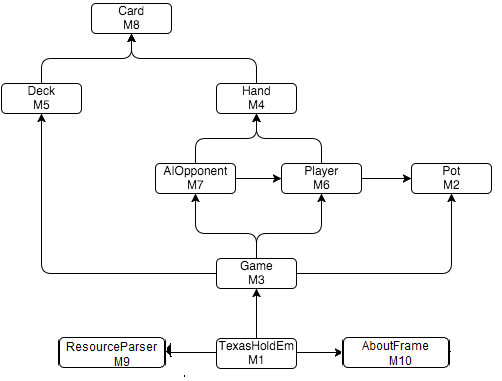
\includegraphics[scale=0.7]{Uses.png}
		\caption{Use Hierarchy Diagram}
		\label{fig1: Figure1}
		\end{figure}
    \section{Traceability Matrix}
    \section{Schedule}
        
    \end{document}